\documentclass[12pt]{report}

\usepackage[a4paper]{geometry}
\usepackage[myheadings]{fullpage}
\usepackage{fancyhdr}
\usepackage{lastpage}
\usepackage{graphicx, wrapfig, subcaption, setspace, booktabs}
\usepackage[T1]{fontenc}
\usepackage[font=small, labelfont=bf]{caption}
\usepackage{fourier}
\usepackage[protrusion=true, expansion=true]{microtype}

%Paquete para hipervinculos
\usepackage[colorlinks=true]{hyperref}
\hypersetup{
    colorlinks=true,
    linkcolor=black,
    filecolor=magenta,      
    urlcolor=blue,
}

%Para qué los subtítulos aparezcan en español
\usepackage[english]{babel}
\usepackage[utf8]{inputenc}
\usepackage{sectsty}
\usepackage{url, lipsum}
\usepackage{tabularx}
\usepackage{float}

%--------------------------------------------------
%Para agregar citas en apa
%Para citar se usa el comando \cite{}
%Las referencias se modifican en el archivo sample.bib
\usepackage{apacite}
%----------------------------------------------

\newcommand{\HRule}[1]{\rule{\linewidth}{#1}}
\onehalfspacing
\setcounter{tocdepth}{5}
\setcounter{secnumdepth}{5}

%-------------------------------------------------------------------------------
%Encabezado y pie de pagina y numeracion
%\fancyhead para encabezado
%\fancyfoot para pie de pagina
% L para izquierda, left
% R para derecha, right
% C para centro, center
%-------------------------------------------------------------------------------
\pagestyle{fancy}
\fancyhf{}
\setlength\headheight{15pt}
\fancyhead[L]{\chaptername \ \thechapter} 
\fancyhead[R]{Université Sidi Mohamed Ben Abdellah}
\fancyfoot[R]{\thepage}

%Le package fncychap propose un ensemble de thèmes déjà prédéfinis pour les chapitres de latex.
%https://borntocode.fr/latex-personnaliser-les-titres-chapter/
\usepackage[Lenny]{fncychap} %[Lenny]/[Sonny]/[Glenn]/[Conny]/[Rejne]

\usepackage{xcolor}
\usepackage{listings}

\definecolor{mGreen}{rgb}{0,0.6,0}
\definecolor{mGray}{rgb}{0.5,0.5,0.5}
\definecolor{mPurple}{rgb}{0.58,0,0.82}
\definecolor{backgroundColour}{rgb}{0.95,0.95,0.92}

\lstdefinestyle{CStyle}{
    backgroundcolor=\color{backgroundColour},   
    commentstyle=\color{mGreen},
    keywordstyle=\color{magenta},
    numberstyle=\tiny\color{mGray},
    stringstyle=\color{mPurple},
    basicstyle=\footnotesize,
    breakatwhitespace=false,         
    breaklines=true,                 
    captionpos=b,                    
    keepspaces=true,                 
    numbers=left,                    
    numbersep=5pt,                  
    showspaces=false,                
    showstringspaces=false,
    showtabs=false,                  
    tabsize=2,
    language=C
}

\begin{document}

\title{ 
        
\includegraphics[width=.5\textwidth]{fsdm.png}~\\[.5cm]
        \normalsize Université Sidi Mohamed Ben            Abdellah \\ 
        USMBA\\
		Faculté de sciences de Fès\\
		FSDM\\
		Laboratoire Informatique, Imagerie et Analyse Numérique\\
		LIIAN
		\\ [2.0cm]
		\HRule{0.5pt} \\
		\LARGE \textbf{Advanced cours completion in C++} %para que quede encerrado en las lineas
		\HRule{2pt} \\ [0.5cm]
		\normalsize \today \vspace*{5\baselineskip}}

\author{Anselme Russel Affane Moundounga}
\date{May 2020}

\maketitle
\tableofcontents

\newpage
\chapter{Introduction}

Programming is an essential tool in the field of scientific research. Indeed, it allows to verify a set of stated theory, to demonstrate postulates through numerical calculation. Traditionally, certain tasks carried out in the context of hypothesis testing are sometimes tedious and still not obvious. This is the case, for example, when it is necessary to perform an iterative and repetitive calculation. Programming tools provide enormous flexibility and save time on certain tasks.

In the field of computer science and programming, there is a multitude of programming languages, those considered low level, i.e. closer to the hardware and sometimes not very obvious like Assembler or C; or those closer to the natural language of the user like Python, R, and so on.

C++ is a programming language located at the border between high level languages and low level languages. Some characteristics of the language are \cite{progcpp}: 

\begin{itemize}
    \item  It is very widespread, it is one of the most widely used programming languages on the planet. So there is a lot of documentation on the Internet and help is easily available on forums. 

    \item It is fast, very fast even, which makes it a language of choice for critical applications that need performance. This is particularly the case for video games, but also for financial tools or certain military programs that need to work in real time.

    \item It is portable, the same source code can theoretically be transformed without problem into executable under Windows, Mac OS and Linux. You will not need to rewrite your program for other platforms.

    \item There are many libraries for C++. Libraries are extensions for the language, a bit like plug-ins. Basically, C++ does not know do a lot, but by combining it with good libraries, you can create 3D, network, audio, windowed, etc. programs.

    \item It is multi-paradigm, which means you can program in C++ in different ways using the Object Oriented Programming (OOP) technique. It is a technique that allows to simplify the organization of the code in our programs and to make it easy to make certain pieces of reusable code.
\end{itemize}


To perform our future scholars and compare results by different way, numerical computing, solver resolution, manual calculation, we decided to use the famous library provide in the 3\(^{dr}\) Numerical Recipes Edition\cite{nr3ed}.


\newpage
\chapter{C Family Syntax}

This chapter is a part of \cite{nr3ed}. Not only C ++ , but also Java, C\#, and (to varying degrees) other computer languages, share a lot of small-scale syntax with the older C language \cite{cppstdlib}. By small scale, we mean operations on built-in types, simple expressions, control structures,
and the like. In this section, we review some of the basics, give some hints on good
programming, and mention some of our conventions and habits.

\section{Operators}

A first piece of advice might seem superfluous if it were not so often ignored:
You should learn all the C operators and their precedence and associativity rules.
You might not yourself want to write

\begin{lstlisting}[style=CStyle]
   n << 1 | 1; 
\end{lstlisting}

as a synonym for 2*n+1 (for positive integer n), but you definitely do need to be able
to see at a glance that
\begin{lstlisting}[style=CStyle]
   n << 1 + 1; 
\end{lstlisting}

is not at all the same thing! Please study the table on the next page while you brush
your teeth every night. While the occasional set of unnecessary parentheses, for
clarity, is hardly a sin, code that is habitually overparenthesized is annoying and hard
to read.
\begin{figure}[!htbp]
	\centering
	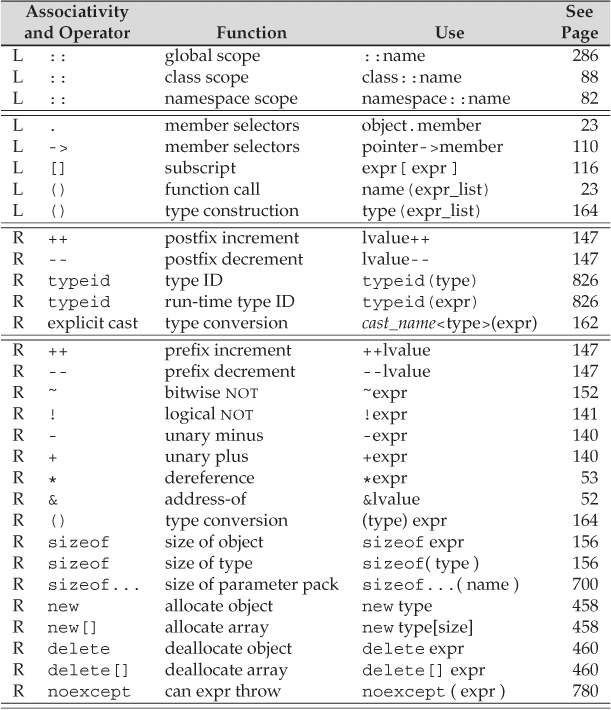
\includegraphics[width=1.\linewidth]{operators.jpg}
	\caption{Operator Precedence and Associativity Rules in C and C ++}
	\label{fig:operatorccpp}
\end{figure}

\newpage
\section{Control Structures}

These should all be familiar to you.

\subsection{Iteration}

In C++ family languages simple iteration is performed with a for loop. In this, we have Initialization, condition and increment as below:
\begin{lstlisting}[style=CStyle]
for (initialisation ; condition ; incrementation)
{
}
\end{lstlisting}

A concret example to display numbers from 0 to 9:

\begin{lstlisting}[style=CStyle]
#include <iostream>
#include "nr3.h" //This our Numerical Recipses 3 main header
using namespace std;//To indicate in which feature set our source file will draw from

Int main()
{
    for (Int compteur(0) ; compteur < 10 ; compteur++)
    {
        cout << compteur << endl;
    }
    return 0;
}
\end{lstlisting}

\subsection{Conditional}

The conditional or if structure looks, in full generality, like
this:
\begin{lstlisting}[style=CStyle]
if (...) {
    ...
}
else if  (...){
    ...
}
else {
    ...
}
\end{lstlisting}

An example: 
\begin{lstlisting}[style=CStyle]
#include <iostream>
#include "nr3.h" //This our Numerical Recipses 3 main header
using namespace std;//To indicate in which feature set our source file will draw from

Int main()
{
    if (b > 3) {
        if (a > 3) b += 1;
    } 
    else {
        b -= 1;
    }
    return 0;
}
\end{lstlisting}

As judged by the indentation used on successive lines, the intent of the writer of this
code is the following: If b is greater than 3 and a is greater than 3, then increment
b. If b is not greater than 3, then decrement b.


\subsection{While iteration}

Iternative to the for iteration is the while structure, for
example: 
\begin{lstlisting}[style=CStyle]
#include <iostream>
#include "nr3.h" //This our Numerical Recipses 3 main header
using namespace std;//To indicate in which feature set our source file will draw from

Int main()
{
    while (n < 1000) {
        n *= 2;
        j += 1;
    }
    return 0;
}
\end{lstlisting}

The control clause (in this case n < 1000) is evaluated before each iteration. If the
clause is not true, the enclosed statements will not be executed. In particular, if this
code is encountered at a time when n is greater than or equal to 1000, the statements
will not even be executed once.

\subsection{Do-While iteration}

Companion to the while iteration is a related control
structure that tests its control clause at the end of each iteration: 
\begin{lstlisting}[style=CStyle]
#include <iostream>
#include "nr3.h" //This our Numerical Recipses 3 main header
using namespace std;//To indicate in which feature set our source file will draw from

Int main()
{
    do {
        n *= 2;
        j += 1;
    } while (n < 1000);
    return 0;
}
\end{lstlisting}

In this case, the enclosed statements will be executed at least once, independent of
the initial value of n.

Your can read deeply \cite{nr3ed} and \cite{progcpp} to get more in C++ programming language.

\newpage
\chapter{Vector and Matrix Objects}
The C ++ Standard Library \cite{cppstdlib} includes a perfectly good vector<> template
class. About the only criticism that one can make of it is that it is so feature-rich that some compiler vendors neglect to squeeze the last little bit of performance out
of its most elementary operations, for example returning an element by its subscript.
That performance is extremely important in scientific applications \cite{nr3ed}!

The result of this history is that C ++ , at least now, has a good (but not always
reliably optimized) class for vectors and no dependable class at all for matrices or
higher-dimensional arrays. What to do? We will adopt a strategy that emphasizes
flexibility and assumes only a minimal set of properties for vectors and matrices.
We will then provide our own, basic, classes for vectors and matrices\cite{nr3ed}. 

For most
compilers, these are at least as efficient as vector<> and other vector and matrix
classes in common use. But if, for you, they’re not, then it is easy to change to a
different set of classes, as we will explain.


\section{C++ Arrays}
\subsection{Static arrays}

\subsubsection{Example 1: }
\begin{lstlisting}[style=CStyle]
#include <iostream>
#include "nr3.h" //This our Numerical Recipses 3 main header
using namespace std;//To indicate in which feature set our source file will draw from

Int main()
{
    Int bestScore[5]; //Declare a table of 5 inters
    Doub anglesTriangle[3]; //Declare a table of  3 doubles
    
    return 0;
}
\end{lstlisting}

\subsubsection{Example 2: }
\begin{lstlisting}[style=CStyle]
#include <iostream>
#include "nr3.h" //This our Numerical Recipses 3 main header
using namespace std;//To indicate in which feature set our source file will draw from

Int main()
{
    Int const tabDim(5); //Dimension of array
    Doub table[tabDim]; 
    
    //Supplying the table
    for (Int i(0); i < tabDim; i++){
        cout << "Enter the " << i+1 << "of the table : ";
        cin >> table[i] <<endl;
    }
    
    //Display the table
    for (Int i(0); i < tabDim; i++){
        cout << table[i] <<endl;
    }
    
    return 0;
}
\end{lstlisting}


\subsubsection{Example 3: Compute the mean }
\begin{lstlisting}[style=CStyle]
#include <iostream>
#include "nr3.h"
using namespace std;

Doub moyenneNotes (Doub tabNotes[], Int dim){
	Doub moyenne(0);
	for(Int i(0); i < dim; i++){
		cout << "Entrer la note " << i+1 << " : ";
		cin >> tabNotes[i];
		
		moyenne += tabNotes[i];
	}
	//moyenne /= dim;
	cout << "La moyenne des notes est : " << endl;
	return (moyenne /= dim);
}

Int main(){
	//Doub listNotes[100];
	Int taille;
	//Doub moyenne(0);
	
	cout << "Saisir le nombre de notes : ";
	cin >> taille;
	Doub listNotes[taille];
	
	//moyenneNotes(listNotes, taille);
	
	cout << moyenneNotes(listNotes, taille) << endl;
	
	return 0;
	
}

\end{lstlisting}

\subsection{C++ Dynamic arrays}
Before to use a dynamic array in C++, we should add \#include<vector> at the beginning of the program. A $vector$ models a dynamic array.

\subsubsection{Example 1 :}
\begin{lstlisting}[style=CStyle]
#include <iostream>
#include <vector> //Don-t forget!
#include "nr3.h"
using namespace std;

Int main(){
	vector<int> table(5);
	return 0;
}

\end{lstlisting}

\subsubsection{Example 2 :}
\begin{lstlisting}[style=CStyle]
#include <iostream>
#include <vector> //Don't forget!
#include "nr3.h"
using namespace std;

Int main(){
	vector<Int> tableau(5, 3); //Creates an array of 5 integers all worth 3
    
    vector<string> listNames(12, "No name"); //Creates an array of 12 strings all worth No name 
    
    vector<Doub> table2; //Creates an array of 0 decimal places
    
	return 0;
}

\end{lstlisting}

\subsection{Abilities of Vectors}
\begin{figure}[!htbp]
	\centering
	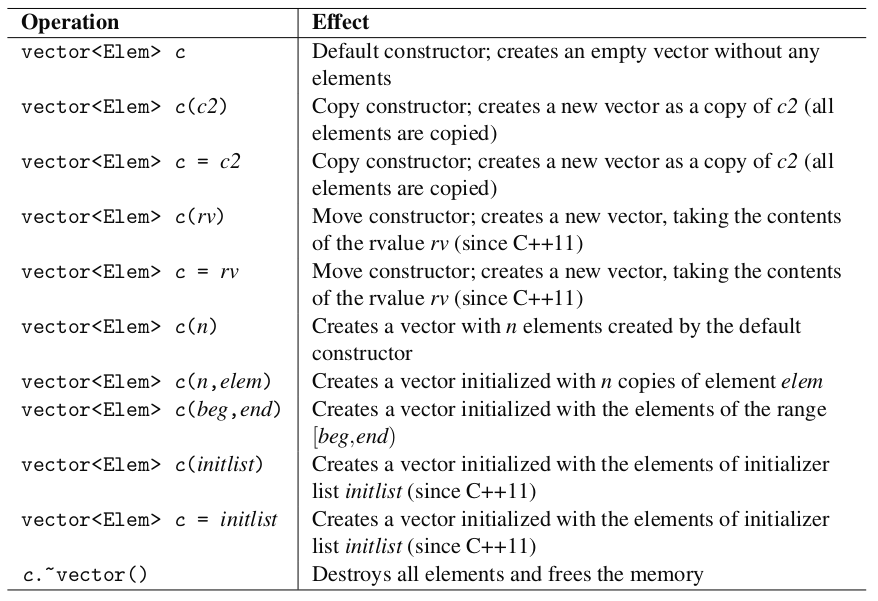
\includegraphics[width=1.\linewidth]{vectoroperation.png}
	\caption{Constructors and Destructor of Vectors}
	\label{fig:constructorofvector}
\end{figure}


\subsection{Vector Operations}
You can create vectors with and without
elements for initialization. If you pass only the size, the elements are created with their default
constructor. Note that an explicit call of the default constructor also initializes fundamental types,
such as int, with zero \cite{cppstdlib}.
\begin{figure}[!htbp]
	\centering
	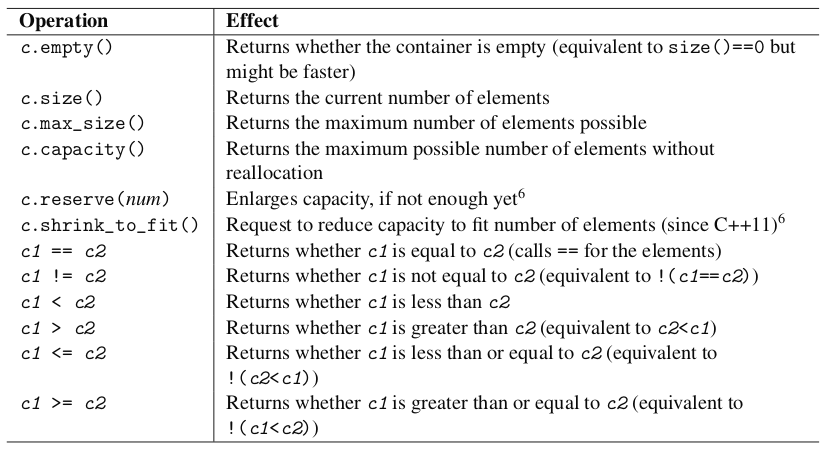
\includegraphics[width=1.\linewidth]{vectoroperation2.png}
	\caption{Nonmodifying Operations of Vectors}
	\label{fig:constructorofvector}
\end{figure}

\subsection{Other example of Using Vectors}
Explicit details into \cite{cppstdlib}.

\begin{lstlisting}[style=CStyle]
#include <vector>
#include <iostream>
#include <string>
#include <algorithm>
#include <iterator>
using namespace std;

int main()
{
    // create empty vector for strings
    vector<string> sentence;

    // reserve memory for five elements to avoid reallocation
    sentence.reserve(5);

    // append some elements
    sentence.push_back("Hello,");
    sentence.insert(sentence.end(),{"how","are","you","?"});

    // print elements separated with spaces
    copy (sentence.cbegin(), sentence.cend(),
          ostream_iterator<string>(cout," "));
    cout << endl;

    // print "technical data"
    cout << "  max_size(): " << sentence.max_size() << endl;
    cout << "  size():     " << sentence.size()     << endl;
    cout << "  capacity(): " << sentence.capacity() << endl;

    // swap second and fourth element
    swap (sentence[1], sentence[3]);

    // insert element "always" before element "?"
    sentence.insert (find(sentence.begin(),sentence.end(),"?"),
                     "always");

    // assign "!" to the last element
    sentence.back() = "!";
    
    // print elements separated with spaces
    copy (sentence.cbegin(), sentence.cend(),
          ostream_iterator<string>(cout," "));
    cout << endl;

    // print some "technical data" again
    cout << "  size():     " << sentence.size()     << endl;
    cout << "  capacity(): " << sentence.capacity() << endl;

    // delete last two elements
    sentence.pop_back();
    sentence.pop_back();
    // shrink capacity (since C++11)
    sentence.shrink_to_fit();

    // print some "technical data" again
    cout << "  size():     " << sentence.size()     << endl;
    cout << "  capacity(): " << sentence.capacity() << endl;
}


\end{lstlisting}

\section{NR3 Typedefs}
With numerical recipes, the flexibility is achieved by having several layers of typedef type-indirection,
resolved at compile time so that there is no run-time performance penalty. The first
level of type-indirection, not just for vectors and matrices but for virtually all vari-
ables, is that we use user-defined type names instead of C ++ fundamental types.
These are defined in \textbf{nr3.h}. The
complete list of such definitions is below, \ref{fig:NRTypedef} \cite{nr3ed}.

\begin{figure}[!htbp]
	\centering
	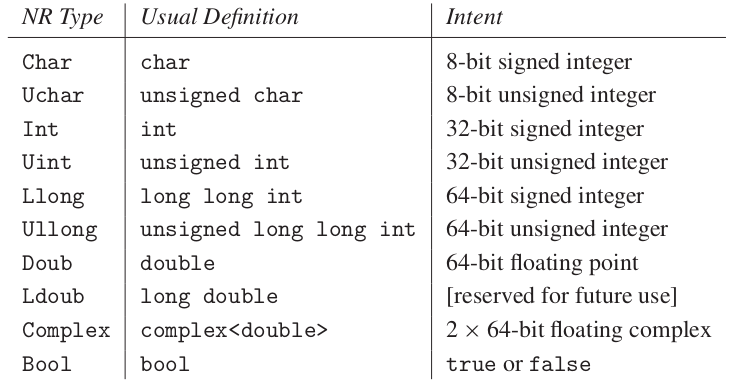
\includegraphics[width=1.\linewidth]{NR_Typedef.png}
	\caption{Numerical Recipes Typedef}
	\label{fig:NRTypedef}
\end{figure}

\subsection{NR3 Typedef: Int, Doub, Char types} 

\subsubsection{EXAMPLE 1 : Square of n.}

\begin{lstlisting}[style=CStyle]
#include <iostream>
#include "nr3.h"
using namespace std;

Int leCarre(Int x){
	/*Int carre(0);
	carre = x * x;
	return carre;*/
	return x * x;
}

Int main(){
	Int x;
	cout << "Entrer un nombre (x) : ";
	cin >> x;
	cout << "x^2 = " << leCarre(x) << endl;
	return 0; 
}
}
\end{lstlisting}

\subsubsection{EXAMPLE 2 : Summation of a and b.}

\begin{lstlisting}[style=CStyle]
#include <iostream>
#include "nr3.h"
using namespace std;

Int addition(Int a, Int b){		
		return a + b;
}

Int main(){
		Doub nbr1(0), nbr2(0), nbr3(0);
		cout << "Saisir le nombre 1 : ";
		cin >> nbr1;
		cout << "Saisir le nombre 2 : ";
		cin >> nbr2;
		cout << "Saisir le nombre 3 : ";
		cin >> nbr3;
		cout << " Le produit de " << nbr1 << " par " << nbr2 << " et par " << nbr3 << " = " << multiplication(nbr1, nbr2, nbr3) << endl;
		
		return 0; 
}

\end{lstlisting}

\subsubsection{EXAMPLE 3 : Multiplication a by b.}

\begin{lstlisting}[style=CStyle]
#include <iostream>
#include "nr3.h"
using namespace std;

Doub multiplication(Doub a, Doub b, Doub c){
	return a * b * c;
}

Int main(){
		Doub nbr1(0), nbr2(0), nbr3(0);
		cout << "Saisir le nombre 1 : ";
		cin >> nbr1;
		cout << "Saisir le nombre 2 : ";
		cin >> nbr2;
		cout << "Saisir le nombre 3 : ";
		cin >> nbr3;
		cout << " Le produit de " << nbr1 << " par " << nbr2 << " et par " << nbr3 << " = " << multiplication(nbr1, nbr2, nbr3) << endl;
		
		return 0; 
}

\subsubsection{EXAMPLE 4 : Area of the rectangle.}

\begin{lstlisting}[style=CStyle]
#include <iostream>
#include "nr3.h"
using namespace std;

Int surfaceRectange(Int L, Int l){
	Int s(0);
	if(L >= 0 && l >= 0)
		s = L*l;
	
	return s;
}

Int main(){
	Int longueur, largeur;
	
	cout << "Saisir la longueur du rectange : ";
	cin >> longueur;
	cout << "Saisir la hauteur du rectange : ";
	cin >> largeur;
	
	cout << "La surface du rectangle (s = L * l) est : " << surfaceRectange(longueur, largeur) << " m^2 " << endl;
	//surfaceRectange(longueur, largeur);
	
	return 0;
	
}
\end{lstlisting}

\subsubsection{EXAMPLE 5 : Add 2 to n.}

\begin{lstlisting}[style=CStyle]
#include <iostream>
#include "nr3.h"
using namespace std;

//Int ajoutDeux(Int a){
Int ajoutDeux(Int& a){ //passage par reference
	a += 2; // ==> a = a + 2;
		
	return a;
}

Int main(){
		Int nbr(0), resultat(0);
		cout << "Saisir un nombre : ";
		cin >> nbr;
		
		resultat = ajoutDeux(nbr);
		
		cout <<"Le nombre fourni est : " << nbr << endl;
		cout <<"Le resultat vaut : " << resultat << endl;
		
		return 0; 
}

\end{lstlisting}

\subsection{NR3 Typedef: VecInt, VecDoub, VecChar types}
The second level of type-indirection returns us to \textbf{the discussion of vectors and
matrices}. The vector and matrix types that appear in Numerical Recipes source
code are as follows. 
\begin{itemize}
    \item \textbf{Vectors}: VecInt, VecUint, VecChar, VecUchar, VecCharp,
VecLlong, VecUllong, VecDoub, VecDoubp, VecComplex, and VecBool.

    \item \textbf{Matrices}: MatInt, MatUint, MatChar, MatUchar, MatLlong, MatUllong, MatDoub,
MatComplex, and MatBool. 
\end{itemize}


\textbf{NB}: These should all be understandable, semantically, as
vectors and matrices whose elements are the corresponding user-defined types, above. Those ending in a “p” have elements that are pointers, e.g., VecCharp is a vector of
pointers to char, that is, char*.

\subsubsection{EXAMPLE 1 : Vectors.}

\begin{lstlisting}[style=CStyle]
#include <iostream>
#include "nr3.h"
using namespace std;

Int main(){
	VecDoub a(10);
	
	for(Int i(0); i < a.size(); i++){
		cout << "Saisir la valeur " << i+1 << " du tableau ";
		cin >> a[i];
	}
	cout << "V(i) = " ;
	cout << "{ ";
	for(Int i(0); i < a.size(); i++){
		cout << a[i];
		if(i < 9) 
			cout << ", ";
	} 
	cout << "} " << endl;
	return 0;
}

\end{lstlisting}

\subsubsection{EXAMPLE 2 : Matrices.}

\begin{lstlisting}[style=CStyle]
#include <iostream>
#include "nr3.h"
using namespace std;

Int main(){
	Int l(3), c(4);
	MatDoub matrix(l, c);
	
	for(Int i(0); i < l; i++){
		for (Int j(0); j < c; j++){
			cout << "Saisir l'element [" << i << "][" << j << "] de la matrice ";
			cin >> matrix[i][j];
		}
	}
	cout << "Matrix[l][c] = " << "{ "<<  endl;
	for(Int i(0); i < l; i++){
		for (Int j(0); j < c; j++){
			cout << matrix[i][j]<<  ", ";			
		}
		cout <<  endl;
	} 
	cout << "} " << endl;
	return 0;
}

\end{lstlisting}

\newpage
%-------------------------------------------------------------------------------
% REFERENCIAS
%-------------------------------------------------------------------------------

\bibliographystyle{apacite}
\bibliography{ref.bib}
%\begin{thebibliography}{00}
%\bibitem{b1} 
%\end{thebibliography}
\end{document}
